
\begin{frame}
\todo{JERC}

\todo{custom loss}

\end{frame}

\subsection*{The standard model}
\begin{frame}
\frametitle{The Standard Model}
\begin{center}
\ifdefined\homedir \else \def\homedir{/home/torterotot}\fi
\IfFileExists{\homedir/Dropbox/Enseignement/TikZ_files/modele_standard_EN/init.tex}{
\includegraphics[scale=.575]{\PhDthesisdir/tex/slides/SM_MSSM_HTT_pheno/SM_and_its_limits/_SM2018.tex}
}{
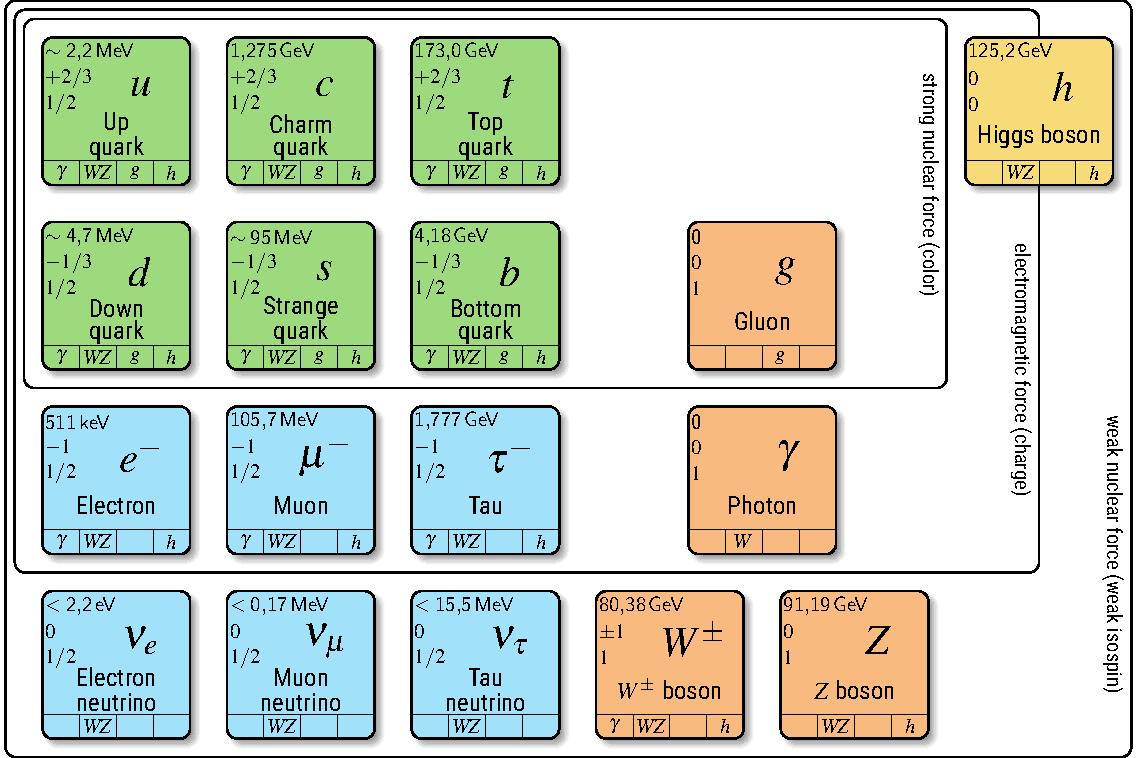
\includegraphics[scale=.575]{\PhDthesisdir/tex/slides/SM_MSSM_HTT_pheno/SM_and_its_limits/SM_2018-bak.pdf}
}
\end{center}
\end{frame}

\begin{frame}
\frametitle{The Standard Model and naturalness problem}

\manip Higgs mass measured: $m_{\higgs} = \num{125.10} \pm \SI{0.14}{\GeV}$\beamercite{PDG_booklet_2020}

\manip Higgs mass derivation:
$\displaystyle
m_{\higgs}^2 = m_{\higgs 0}^2 -\frac{3}{8\pi^2} y_{\quarkt}^2 \Lambda^2  +\frac{1}{16\pi^2} g^2 \Lambda^2 + \frac{1}{16\pi^2} \lambda^2 \Lambda^2 + \ldots
$

\begin{minipage}[t]{.3\textwidth}
\begin{block}{top quark}
\begin{center}
\vspace{-4.5pt}
\begin{fmffile}{Higgs_loop_fermion}\fmfstraight
\begin{fmfchar*}(30,20)
  \fmfleft{i}
  \fmfright{o}
  \fmf{dashes}{i,v1}
  \fmf{dashes}{v2,o}
  \fmf{fermion,left,tension=.3}{v1,v2,v1}
  \fmfdot{v1,v2}
  \fmflabel{ }{i}
\end{fmfchar*}
\end{fmffile}

\vspace{-4.5pt}

$\displaystyle -\frac{3}{8\pi^2} y_{\quarkt}^2 \Lambda^2 \sim -(\SI{2}{\TeV})^2$
\end{center}
\end{block}
\end{minipage}
\hfill
\begin{minipage}[t]{.3\textwidth}
\begin{block}{vector bosons}
\begin{center}
\begin{fmffile}{Higgs_loop_gauge}\fmfstraight
\begin{fmfchar*}(30,20)
  \fmfleftn{i}{4}
  \fmfrightn{o}{4}
  \fmf{dashes}{i2,v,o2}
  \fmf{phantom}{i4,vbis,o4}
  \fmffreeze
  \fmf{boson, right}{v,vbis,v}
  \fmfdot{v}
  \fmflabel{ }{i2}
\end{fmfchar*}
\end{fmffile}

\vspace{-9pt}

$\displaystyle +\frac{1}{16\pi^2} g^2 \Lambda^2 \sim +(\SI{0.7}{\TeV})^2$
\end{center}
\end{block}
\end{minipage}
\hfill
\begin{minipage}[t]{.3\textwidth}
\begin{block}{Higgs itself}
\begin{center}
\begin{fmffile}{Higgs_loop_sfermion}\fmfstraight
\begin{fmfchar*}(30,20)
  \fmfleftn{i}{4}
  \fmfrightn{o}{4}
  \fmf{dashes}{i2,v,o2}
  \fmf{phantom}{i4,vbis,o4}
  \fmffreeze
  \fmf{dashes, right}{v,vbis,v}
  \fmfdot{v}
  \fmflabel{ }{i2}
\end{fmfchar*}
\end{fmffile}

\vspace{-9pt}

$\displaystyle + \frac{1}{16\pi^2} \lambda^2 \Lambda^2 \sim +(\SI{0.5}{\TeV})^2$
\end{center}
\end{block}
\end{minipage}

\end{frame}

\begin{frame}
\frametitle{Supersymmetry}

\begin{minipage}[t]{.3\textwidth}
\begin{block}{top quark}
\begin{center}
\vspace{-4.5pt}
\begin{fmffile}{Higgs_loop_fermion}\fmfstraight
\begin{fmfchar*}(30,20)
  \fmfleft{i}
  \fmfright{o}
  \fmf{dashes}{i,v1}
  \fmf{dashes}{v2,o}
  \fmf{fermion,left,tension=.3}{v1,v2,v1}
  \fmfdot{v1,v2}
  \fmflabel{ }{i}
\end{fmfchar*}
\end{fmffile}

\vspace{-4.5pt}

$\sim -(\SI{2}{\TeV})^2$
\end{center}
\end{block}
\end{minipage}
\hfill
\begin{minipage}[t]{.3\textwidth}
\begin{block}{vector bosons}
\begin{center}
\begin{fmffile}{Higgs_loop_gauge}\fmfstraight
\begin{fmfchar*}(30,20)
  \fmfleftn{i}{4}
  \fmfrightn{o}{4}
  \fmf{dashes}{i2,v,o2}
  \fmf{phantom}{i4,vbis,o4}
  \fmffreeze
  \fmf{boson, right}{v,vbis,v}
  \fmfdot{v}
  \fmflabel{ }{i2}
\end{fmfchar*}
\end{fmffile}

\vspace{-9pt}

$\sim +(\SI{0.7}{\TeV})^2$
\end{center}
\end{block}
\end{minipage}
\hfill
\begin{minipage}[t]{.3\textwidth}
\begin{block}{Higgs itself}
\begin{center}
\begin{fmffile}{Higgs_loop_sfermion}\fmfstraight
\begin{fmfchar*}(30,20)
  \fmfleftn{i}{4}
  \fmfrightn{o}{4}
  \fmf{dashes}{i2,v,o2}
  \fmf{phantom}{i4,vbis,o4}
  \fmffreeze
  \fmf{dashes, right}{v,vbis,v}
  \fmfdot{v}
  \fmflabel{ }{i2}
\end{fmfchar*}
\end{fmffile}

\vspace{-9pt}

$\sim +(\SI{0.5}{\TeV})^2$
\end{center}
\end{block}
\end{minipage}


\begin{minipage}[t]{.3\textwidth}
\begin{block}{stop quark}
\begin{center}
\begin{fmffile}{Higgs_loop_sfermion}\fmfstraight
\begin{fmfchar*}(30,20)
  \fmfleftn{i}{4}
  \fmfrightn{o}{4}
  \fmf{dashes}{i2,v,o2}
  \fmf{phantom}{i4,vbis,o4}
  \fmffreeze
  \fmf{dashes, right}{v,vbis,v}
  \fmfdot{v}
  \fmflabel{ }{i2}
\end{fmfchar*}
\end{fmffile}

\vspace{-9pt}

$\sim +(\SI{2}{\TeV})^2$
\end{center}
\end{block}
\end{minipage}
\hfill
\begin{minipage}[t]{.3\textwidth}
\begin{block}{bosinos}
\begin{center}
\vspace{-4.5pt}
\begin{fmffile}{Higgs_loop_fermion}\fmfstraight
\begin{fmfchar*}(30,20)
  \fmfleft{i}
  \fmfright{o}
  \fmf{dashes}{i,v1}
  \fmf{dashes}{v2,o}
  \fmf{fermion,left,tension=.3}{v1,v2,v1}
  \fmfdot{v1,v2}
  \fmflabel{ }{i}
\end{fmfchar*}
\end{fmffile}

\vspace{-4.5pt}

$\sim -(\SI{0.7}{\TeV})^2$
\end{center}
\end{block}
\end{minipage}
\hfill
\begin{minipage}[t]{.3\textwidth}
\begin{block}{Higgsinos}
\begin{center}
\vspace{-4.5pt}
\begin{fmffile}{Higgs_loop_fermion}\fmfstraight
\begin{fmfchar*}(30,20)
  \fmfleft{i}
  \fmfright{o}
  \fmf{dashes}{i,v1}
  \fmf{dashes}{v2,o}
  \fmf{fermion,left,tension=.3}{v1,v2,v1}
  \fmfdot{v1,v2}
  \fmflabel{ }{i}
\end{fmfchar*}
\end{fmffile}

\vspace{-4.5pt}

$\sim -(\SI{0.5}{\TeV})^2$
\end{center}
\end{block}
\end{minipage}

\end{frame}

%\begin{frame}
%\frametitle{Naturalness and supersymmetry}
%\manip Higgs mass: $\displaystyle m_{\higgs}^{2}=2\mu ^{2}+\delta m_{\higgs}^{2} \simeq \SI{125}{\GeV}$
%\begin{equation*}
%\delta m_{\higgs}^{2}\simeq {\frac {3}{4\pi ^{2}}}{\Bigl (}-\lambda _{\quarkt}^{2}+{\frac {g^{2}}{4}}+{\frac {g^{2}}{8\cos ^{2}\theta _{W}}}+\lambda {\Bigr )}\Lambda ^{2}
%\end{equation*}
%
%For instance, if one includes see-saw neutrinos into the Standard Model, then $\delta m_{\higgs}$ would blow up to near the see-saw scale, typically expected in the \SI{e13}{\GeV} range. 
%
%\end{frame}
%
%\begin{frame}
%\frametitle{Naturalness and supersymmetry}
%\manip By supersymmetrizing the Standard Model, one arrives at a solution to the gauge hierarchy, or big hierarchy, problem in that supersymmetry guarantees cancellation of quadratic divergences to all orders in perturbation theory.
%
%\begin{fmffile}{Higgs_loop_fermion}\fmfstraight
\begin{fmfchar*}(30,20)
  \fmfleft{i}
  \fmfright{o}
  \fmf{dashes}{i,v1}
  \fmf{dashes}{v2,o}
  \fmf{fermion,left,tension=.3}{v1,v2,v1}
  \fmfdot{v1,v2}
  \fmflabel{ }{i}
\end{fmfchar*}
\end{fmffile}

%
%\begin{fmffile}{Higgs_loop_sfermion}\fmfstraight
\begin{fmfchar*}(30,20)
  \fmfleftn{i}{4}
  \fmfrightn{o}{4}
  \fmf{dashes}{i2,v,o2}
  \fmf{phantom}{i4,vbis,o4}
  \fmffreeze
  \fmf{dashes, right}{v,vbis,v}
  \fmfdot{v}
  \fmflabel{ }{i2}
\end{fmfchar*}
\end{fmffile}

%
%\end{frame}

\begin{frame}
\frametitle{2 Higgs doublets models for supersymmetry}
\begin{equation*}
\average{\phi_1}_0 = \frac{1}{\sqrt{2}} \begin{pmatrix}
0\\v_1
\end{pmatrix}
\msep
\average{\phi_2}_0 = \frac{1}{\sqrt{2}} \begin{pmatrix}
0\\v_2 \eexp{\im\xi}
\end{pmatrix}
\end{equation*}

\begin{equation*}
\boxed{\tan\beta = \frac{\average{\phi_2}_0}{\average{\phi_1}_0} = \frac{v_2}{v_1}}
\end{equation*}

\beamercite{Higgs_hunter_guide}
\end{frame}

\subsection*{Why histograms}
\begin{frame}
\frametitle{Using histograms}

\manip Find a discriminating variable:
\submanip for uncorrelated \tau\ pairs, it's random
\submanip for \tau\ pairs coming from a particle (Higgs?), not random.

\manip For one \tau\ pair only, impossible to say!

\manip With many events, a difference may show up.
\end{frame}

\begin{frame}
\frametitle{The rabbit analogy}
\beamercite{Higgs_discovery_explained_video_3}

\manip White rabbit that once lived in a casino.
\submanip The rabbit loved watching people playing dices.
\submanip He was happy when the result of dice was 4.
\submanip So when he sees a dice, he turns it so that the result is 4.
\submanip But this rabbit is very shy and nobody has seen him since the casino closure.
\submanip The only way to know if he's here is to throw a dice and come back to see the result.
\submanip If the rabbit has been here, the dice will show a 4!
\end{frame}

\begin{frame}
\frametitle{The rabbit analogy}
\beamercite{Higgs_discovery_explained_video_3}

\manip Dice results:
4\pause,
2\pause,
4,
1,
3,
2,
5,
1,
1,
6...
\end{frame}

\begin{frame}
\frametitle{The rabbit analogy}
\beamercite{Higgs_discovery_explained_video_3}
\begin{center}
\begin{minipage}[c]{.29\textwidth}
On \num{100} days $\rightarrow$
\end{minipage}
\begin{minipage}[c]{.4\textwidth}
\vspace{-\baselineskip}
\includegraphics[height=\graphh, width=\graphw,keepaspectratio]{/home/torterotot/Documents/PhD-Thesis/plots_and_images/my_plots/inspired_from_Higgs_discovery_explained_video_3/1-only_data_100-pyplot.tex}
\end{minipage}
\begin{minipage}[c]{.29\textwidth}
Not really conclusive...
\end{minipage}
\end{center}
\end{frame}

\begin{frame}
\frametitle{The rabbit analogy}
\addtocounter{framenumber}{-1}
\beamercite{Higgs_discovery_explained_video_3}
\begin{center}
\begin{minipage}[c]{.29\textwidth}
On \num{100} days $\rightarrow$
\end{minipage}
\begin{minipage}[c]{.4\textwidth}
\vspace{-\baselineskip}
\includegraphics[height=\graphh, width=\graphw,keepaspectratio]{/home/torterotot/Documents/PhD-Thesis/plots_and_images/my_plots/inspired_from_Higgs_discovery_explained_video_3/2-data_and_bg_estim_100-pyplot.tex}
\end{minipage}
\begin{minipage}[c]{.29\textwidth}
Comparing with predictions!
\end{minipage}
\end{center}
\end{frame}

\begin{frame}
\frametitle{The rabbit analogy}
\addtocounter{framenumber}{-1}
\beamercite{Higgs_discovery_explained_video_3}
\begin{center}
\begin{minipage}[c]{.29\textwidth}
On \num{100} days $\rightarrow$
\end{minipage}
\begin{minipage}[c]{.4\textwidth}
\vspace{-\baselineskip}
\includegraphics[height=\graphh, width=\graphw,keepaspectratio]{/home/torterotot/Documents/PhD-Thesis/plots_and_images/my_plots/inspired_from_Higgs_discovery_explained_video_3/3-data_and_bg_estim_ratio_100-pyplot.tex}
\end{minipage}
\begin{minipage}[c]{.29\textwidth}
Also add ratio plot:\\
observed / predictions
\end{minipage}
\end{center}
\end{frame}

\begin{frame}
\frametitle{The rabbit analogy}
\addtocounter{framenumber}{-1}
\beamercite{Higgs_discovery_explained_video_3}
\begin{center}
\begin{minipage}[c]{.29\textwidth}
On \num{100} days $\rightarrow$
\end{minipage}
\begin{minipage}[c]{.4\textwidth}
\vspace{-\baselineskip}
\includegraphics[height=\graphh, width=\graphw,keepaspectratio]{/home/torterotot/Documents/PhD-Thesis/plots_and_images/my_plots/inspired_from_Higgs_discovery_explained_video_3/4-up_to_100-pyplot.tex}
\end{minipage}
\begin{minipage}[c]{.29\textwidth}
Fill up with more data!
\end{minipage}
\end{center}
\end{frame}

%\begin{frame}
%\frametitle{The rabbit analogy}
%\addtocounter{framenumber}{-1}
%\transwipe[direction=90]
%\beamercite{Higgs_discovery_explained_video_3}
%\begin{center}
%\begin{minipage}[c]{.29\textwidth}
%On \num{500} days $\rightarrow$
%\end{minipage}
%\begin{minipage}[c]{.4\textwidth}
%\vspace{-\baselineskip}
%\includegraphics[height=\graphh, width=\graphw,keepaspectratio]{/home/torterotot/Documents/PhD-Thesis/plots_and_images/my_plots/inspired_from_Higgs_discovery_explained_video_3/5-up_to_500-pyplot.tex}
%\end{minipage}
%\begin{minipage}[c]{.29\textwidth}
%Fill up with more data!
%\end{minipage}
%\end{center}
%\end{frame}

\begin{frame}
\frametitle{The rabbit analogy}
\addtocounter{framenumber}{-1}
\transwipe[direction=90]
\beamercite{Higgs_discovery_explained_video_3}
\begin{center}
\begin{minipage}[c]{.29\textwidth}
On \num{1000} days $\rightarrow$
\end{minipage}
\begin{minipage}[c]{.4\textwidth}
\vspace{-\baselineskip}
\includegraphics[height=\graphh, width=\graphw,keepaspectratio]{/home/torterotot/Documents/PhD-Thesis/plots_and_images/my_plots/inspired_from_Higgs_discovery_explained_video_3/6-up_to_1000-pyplot.tex}
\end{minipage}
\begin{minipage}[c]{.29\textwidth}
Fill up with more data!
\end{minipage}
\end{center}
\end{frame}

%\begin{frame}
%\frametitle{The rabbit analogy}
%\addtocounter{framenumber}{-1}
%\transwipe[direction=90]
%\transduration{0}
%\beamercite{Higgs_discovery_explained_video_3}
%\begin{center}
%\begin{minipage}[c]{.29\textwidth}
%On \num{1500} days $\rightarrow$
%\end{minipage}
%\begin{minipage}[c]{.4\textwidth}
%\vspace{-\baselineskip}
%\includegraphics[height=\graphh, width=\graphw,keepaspectratio]{/home/torterotot/Documents/PhD-Thesis/plots_and_images/my_plots/inspired_from_Higgs_discovery_explained_video_3/7-up_to_1500-pyplot.tex}
%\end{minipage}
%\begin{minipage}[c]{.29\textwidth}
%Fill up with more data!
%\end{minipage}
%\end{center}
%\end{frame}

\begin{frame}
\frametitle{The rabbit analogy}
\addtocounter{framenumber}{-1}
\transwipe[direction=90]
\transduration{0}
\beamercite{Higgs_discovery_explained_video_3}
\begin{center}
\begin{minipage}[c]{.29\textwidth}
On \num{2000} days $\rightarrow$
\end{minipage}
\begin{minipage}[c]{.4\textwidth}
\vspace{-\baselineskip}
\includegraphics[height=\graphh, width=\graphw,keepaspectratio]{/home/torterotot/Documents/PhD-Thesis/plots_and_images/my_plots/inspired_from_Higgs_discovery_explained_video_3/8-up_to_2000-pyplot.tex}
\end{minipage}
\begin{minipage}[c]{.29\textwidth}
Fill up with more data!
\end{minipage}
\end{center}
\end{frame}

%\begin{frame}
%\frametitle{The rabbit analogy}
%\addtocounter{framenumber}{-1}
%\transwipe[direction=90]
%\transduration{0}
%\beamercite{Higgs_discovery_explained_video_3}
%\begin{center}
%\begin{minipage}[c]{.29\textwidth}
%On \num{2500} days $\rightarrow$
%\end{minipage}
%\begin{minipage}[c]{.4\textwidth}
%\vspace{-\baselineskip}
%\includegraphics[height=\graphh, width=\graphw,keepaspectratio]{/home/torterotot/Documents/PhD-Thesis/plots_and_images/my_plots/inspired_from_Higgs_discovery_explained_video_3/9-up_to_2500-pyplot.tex}
%\end{minipage}
%\begin{minipage}[c]{.29\textwidth}
%Fill up with more data!
%\end{minipage}
%\end{center}
%\end{frame}

\begin{frame}
\frametitle{The rabbit analogy}
\addtocounter{framenumber}{-1}
\transwipe[direction=90]
\transduration{0}
\beamercite{Higgs_discovery_explained_video_3}
\begin{center}
\begin{minipage}[c]{.29\textwidth}
On \num{3000} days $\rightarrow$
\end{minipage}
\begin{minipage}[c]{.4\textwidth}
\vspace{-\baselineskip}
\includegraphics[height=\graphh, width=\graphw,keepaspectratio]{/home/torterotot/Documents/PhD-Thesis/plots_and_images/my_plots/inspired_from_Higgs_discovery_explained_video_3/10-up_to_3000-pyplot.tex}
\end{minipage}
\begin{minipage}[c]{.29\textwidth}
Fill up with more data!
\end{minipage}
\end{center}
\end{frame}

%\begin{frame}
%\frametitle{The rabbit analogy}
%\addtocounter{framenumber}{-1}
%\transwipe[direction=90]
%\transduration{0}
%\beamercite{Higgs_discovery_explained_video_3}
%\begin{center}
%\begin{minipage}[c]{.29\textwidth}
%On \num{3500} days $\rightarrow$
%\end{minipage}
%\begin{minipage}[c]{.4\textwidth}
%\vspace{-\baselineskip}
%\includegraphics[height=\graphh, width=\graphw,keepaspectratio]{/home/torterotot/Documents/PhD-Thesis/plots_and_images/my_plots/inspired_from_Higgs_discovery_explained_video_3/11-up_to_3500-pyplot.tex}
%\end{minipage}
%\begin{minipage}[c]{.29\textwidth}
%Fill up with more data!
%\end{minipage}
%\end{center}
%\end{frame}

\begin{frame}
\frametitle{The rabbit analogy}
\addtocounter{framenumber}{-1}
\transwipe[direction=90]
\transduration{0}
\beamercite{Higgs_discovery_explained_video_3}
\begin{center}
\begin{minipage}[c]{.29\textwidth}
On \num{4000} days $\rightarrow$
\end{minipage}
\begin{minipage}[c]{.4\textwidth}
\vspace{-\baselineskip}
\includegraphics[height=\graphh, width=\graphw,keepaspectratio]{/home/torterotot/Documents/PhD-Thesis/plots_and_images/my_plots/inspired_from_Higgs_discovery_explained_video_3/12-up_to_4000-pyplot.tex}
\end{minipage}
\begin{minipage}[c]{.29\textwidth}
Fill up with more data!
\end{minipage}
\end{center}
\end{frame}

%\begin{frame}
%\frametitle{The rabbit analogy}
%\addtocounter{framenumber}{-1}
%\transwipe[direction=90]
%\transduration{0}
%\beamercite{Higgs_discovery_explained_video_3}
%\begin{center}
%\begin{minipage}[c]{.29\textwidth}
%On \num{4500} days $\rightarrow$
%\end{minipage}
%\begin{minipage}[c]{.4\textwidth}
%\vspace{-\baselineskip}
%\includegraphics[height=\graphh, width=\graphw,keepaspectratio]{/home/torterotot/Documents/PhD-Thesis/plots_and_images/my_plots/inspired_from_Higgs_discovery_explained_video_3/13-up_to_4500-pyplot.tex}
%\end{minipage}
%\begin{minipage}[c]{.29\textwidth}
%Fill up with more data!
%\end{minipage}
%\end{center}
%\end{frame}

\begin{frame}
\frametitle{The rabbit analogy}
\addtocounter{framenumber}{-1}
\transwipe[direction=90]
\transduration{0}
\beamercite{Higgs_discovery_explained_video_3}
\begin{center}
\begin{minipage}[c]{.29\textwidth}
On \num{5000} days $\rightarrow$
\end{minipage}
\begin{minipage}[c]{.4\textwidth}
\vspace{-\baselineskip}
\includegraphics[height=\graphh, width=\graphw,keepaspectratio]{/home/torterotot/Documents/PhD-Thesis/plots_and_images/my_plots/inspired_from_Higgs_discovery_explained_video_3/14-up_to_5000-pyplot.tex}
\end{minipage}
\begin{minipage}[c]{.29\textwidth}
Fill up with more data!
\end{minipage}
\end{center}
\end{frame}

%\begin{frame}
%\frametitle{The rabbit analogy}
%\addtocounter{framenumber}{-1}
%\transwipe[direction=90]
%\transduration{0}
%\beamercite{Higgs_discovery_explained_video_3}
%\begin{center}
%\begin{minipage}[c]{.29\textwidth}
%On \num{5500} days $\rightarrow$
%\end{minipage}
%\begin{minipage}[c]{.4\textwidth}
%\vspace{-\baselineskip}
%\includegraphics[height=\graphh, width=\graphw,keepaspectratio]{/home/torterotot/Documents/PhD-Thesis/plots_and_images/my_plots/inspired_from_Higgs_discovery_explained_video_3/15-up_to_5500-pyplot.tex}
%\end{minipage}
%\begin{minipage}[c]{.29\textwidth}
%Fill up with more data!
%\end{minipage}
%\end{center}
%\end{frame}

\begin{frame}
\frametitle{The rabbit analogy}
\addtocounter{framenumber}{-1}
\transwipe[direction=90]
\transduration{0}
\beamercite{Higgs_discovery_explained_video_3}
\begin{center}
\begin{minipage}[c]{.29\textwidth}
On \num{6000} days $\rightarrow$
\end{minipage}
\begin{minipage}[c]{.4\textwidth}
\vspace{-\baselineskip}
\includegraphics[height=\graphh, width=\graphw,keepaspectratio]{/home/torterotot/Documents/PhD-Thesis/plots_and_images/my_plots/inspired_from_Higgs_discovery_explained_video_3/16-up_to_6000-pyplot.tex}
\end{minipage}
\begin{minipage}[c]{.29\textwidth}
Fill up with more data!
\end{minipage}
\end{center}
\end{frame}

%\begin{frame}
%\frametitle{The rabbit analogy}
%\addtocounter{framenumber}{-1}
%\transwipe[direction=90]
%\transduration{0}
%\beamercite{Higgs_discovery_explained_video_3}
%\begin{center}
%\begin{minipage}[c]{.29\textwidth}
%On \num{6500} days $\rightarrow$
%\end{minipage}
%\begin{minipage}[c]{.4\textwidth}
%\vspace{-\baselineskip}
%\includegraphics[height=\graphh, width=\graphw,keepaspectratio]{/home/torterotot/Documents/PhD-Thesis/plots_and_images/my_plots/inspired_from_Higgs_discovery_explained_video_3/17-up_to_6500-pyplot.tex}
%\end{minipage}
%\begin{minipage}[c]{.29\textwidth}
%Fill up with more data!
%\end{minipage}
%\end{center}
%\end{frame}

\begin{frame}
\frametitle{The rabbit analogy}
\addtocounter{framenumber}{-1}
\transwipe[direction=90]
\transduration{0}
\beamercite{Higgs_discovery_explained_video_3}
\begin{center}
\begin{minipage}[c]{.29\textwidth}
On \num{7000} days $\rightarrow$
\end{minipage}
\begin{minipage}[c]{.4\textwidth}
\vspace{-\baselineskip}
\includegraphics[height=\graphh, width=\graphw,keepaspectratio]{/home/torterotot/Documents/PhD-Thesis/plots_and_images/my_plots/inspired_from_Higgs_discovery_explained_video_3/18-up_to_7000-pyplot.tex}
\end{minipage}
\begin{minipage}[c]{.29\textwidth}
Fill up with more data!
\end{minipage}
\end{center}
\end{frame}

%\begin{frame}
%\frametitle{The rabbit analogy}
%\addtocounter{framenumber}{-1}
%\transwipe[direction=90]
%\transduration{0}
%\beamercite{Higgs_discovery_explained_video_3}
%\begin{center}
%\begin{minipage}[c]{.29\textwidth}
%On \num{7500} days $\rightarrow$
%\end{minipage}
%\begin{minipage}[c]{.4\textwidth}
%\vspace{-\baselineskip}
%\includegraphics[height=\graphh, width=\graphw,keepaspectratio]{/home/torterotot/Documents/PhD-Thesis/plots_and_images/my_plots/inspired_from_Higgs_discovery_explained_video_3/19-up_to_7500-pyplot.tex}
%\end{minipage}
%\begin{minipage}[c]{.29\textwidth}
%Fill up with more data!
%\end{minipage}
%\end{center}
%\end{frame}

\begin{frame}
\frametitle{The rabbit analogy}
\addtocounter{framenumber}{-1}
\transwipe[direction=90]
\transduration{0}
\beamercite{Higgs_discovery_explained_video_3}
\begin{center}
\begin{minipage}[c]{.29\textwidth}
On \num{8000} days $\rightarrow$
\end{minipage}
\begin{minipage}[c]{.4\textwidth}
\vspace{-\baselineskip}
\includegraphics[height=\graphh, width=\graphw,keepaspectratio]{/home/torterotot/Documents/PhD-Thesis/plots_and_images/my_plots/inspired_from_Higgs_discovery_explained_video_3/20-up_to_8000-pyplot.tex}
\end{minipage}
\begin{minipage}[c]{.29\textwidth}
Fill up with more data!
\end{minipage}
\end{center}
\end{frame}

%\begin{frame}
%\frametitle{The rabbit analogy}
%\addtocounter{framenumber}{-1}
%\transwipe[direction=90]
%\transduration{0}
%\beamercite{Higgs_discovery_explained_video_3}
%\begin{center}
%\begin{minipage}[c]{.29\textwidth}
%On \num{8500} days $\rightarrow$
%\end{minipage}
%\begin{minipage}[c]{.4\textwidth}
%\vspace{-\baselineskip}
%\includegraphics[height=\graphh, width=\graphw,keepaspectratio]{/home/torterotot/Documents/PhD-Thesis/plots_and_images/my_plots/inspired_from_Higgs_discovery_explained_video_3/21-up_to_8500-pyplot.tex}
%\end{minipage}
%\begin{minipage}[c]{.29\textwidth}
%Fill up with more data!
%\end{minipage}
%\end{center}
%\end{frame}

\begin{frame}
\frametitle{The rabbit analogy}
\addtocounter{framenumber}{-1}
\transwipe[direction=90]
\transduration{0}
\beamercite{Higgs_discovery_explained_video_3}
\begin{center}
\begin{minipage}[c]{.29\textwidth}
On \num{9000} days $\rightarrow$
\end{minipage}
\begin{minipage}[c]{.4\textwidth}
\vspace{-\baselineskip}
\includegraphics[height=\graphh, width=\graphw,keepaspectratio]{/home/torterotot/Documents/PhD-Thesis/plots_and_images/my_plots/inspired_from_Higgs_discovery_explained_video_3/22-up_to_9000-pyplot.tex}
\end{minipage}
\begin{minipage}[c]{.29\textwidth}
Fill up with more data!
\end{minipage}
\end{center}
\end{frame}

%\begin{frame}
%\frametitle{The rabbit analogy}
%\addtocounter{framenumber}{-1}
%\transwipe[direction=90]
%\transduration{0}
%\beamercite{Higgs_discovery_explained_video_3}
%\begin{center}
%\begin{minipage}[c]{.29\textwidth}
%On \num{9500} days $\rightarrow$
%\end{minipage}
%\begin{minipage}[c]{.4\textwidth}
%\vspace{-\baselineskip}
%\includegraphics[height=\graphh, width=\graphw,keepaspectratio]{/home/torterotot/Documents/PhD-Thesis/plots_and_images/my_plots/inspired_from_Higgs_discovery_explained_video_3/23-up_to_9500-pyplot.tex}
%\end{minipage}
%\begin{minipage}[c]{.29\textwidth}
%Fill up with more data!
%\end{minipage}
%\end{center}
%\end{frame}

\begin{frame}
\frametitle{The rabbit analogy}
\addtocounter{framenumber}{-1}
\transwipe[direction=90]
\beamercite{Higgs_discovery_explained_video_3}
\begin{center}
\begin{minipage}[c]{.29\textwidth}
On \num{10000} days $\rightarrow$
\end{minipage}
\begin{minipage}[c]{.4\textwidth}
\vspace{-\baselineskip}
\includegraphics[height=\graphh, width=\graphw,keepaspectratio]{/home/torterotot/Documents/PhD-Thesis/plots_and_images/my_plots/inspired_from_Higgs_discovery_explained_video_3/24-up_to_10000-pyplot.tex}
\end{minipage}
\begin{minipage}[c]{.29\textwidth}
Fill up with more data!
\end{minipage}
\end{center}
\end{frame}

\begin{frame}
\frametitle{The rabbit analogy}
\addtocounter{framenumber}{-1}
\transdissolve
\beamercite{Higgs_discovery_explained_video_3}
\begin{center}
\begin{minipage}[c]{.29\textwidth}
On \num{10000} days $\rightarrow$
\end{minipage}
\begin{minipage}[c]{.4\textwidth}
\vspace{-\baselineskip}
\includegraphics[height=\graphh, width=\graphw,keepaspectratio]{/home/torterotot/Documents/PhD-Thesis/plots_and_images/my_plots/inspired_from_Higgs_discovery_explained_video_3/25-up_to_10000_SR-pyplot.tex}
\end{minipage}
\begin{minipage}[c]{.29\textwidth}
In red, hypothesis of the rabbit with 3 as preffered result\\
(instead of 4!), with a probability to show up of \SI{5}{\%}.
\end{minipage}
\end{center}
\end{frame}
